
\begin{frame}{‌کوتاهترین مسیر از یک مبدأ}
\begin{itemize}\itemr
\item[-]
فرض کنید می‌خواهیم از شهری به شهر دیگر برویم و برای کاهش هزینه می‌خواهیم کوتاهترین مسیر را انتخاب کنیم.
اطلاعات همهٔ راه‌ها و شهرها و فاصلهٔ بین شهر‌ها را در اختیار داریم. چگونه می‌توانیم با این اطلاعات کوتاهترین مسیر را انتخاب کنیم؟
\item[-]
یک راه ساده این است که همهٔ مسیرها را به دست آورده و طول آنها را با یکدیگر مقایسه کنیم، اما زمان لازم برای انجام چنین الگوریتم آنقدر زیاد است که در عمل مورد استفاده نیست.
\item[-]
در اینجا الگوریتمی برای محاسبهٔ جواب این مسئله به طور کارامد ارائه می‌کنیم.
\end{itemize}
\end{frame}


\begin{frame}{‌کوتاهترین مسیر از یک مبدأ}
\begin{itemize}\itemr
\item[-]
ورودی مسئلهٔ کوتاهترین مسیر
\fn{1}{shortest path problem},
گراف جهت‌دار وزن‌دار
\m{G = (V,E)}
با تابع وزن
\m{w : E \rightarrow \RR}
است که به ازای هر یال وزن آن را باز می‌گرداند. وزن مسیر
\m{p = \langle v_0,v_1, \cdots , v_k \rangle}
که به صورت
\m{w(p)}
نشان داده می‌شود برابراست با مجموع وزن همهٔ یال‌های مسیر:
\begin{align*}
\m{w(p) = \sum_{i = 1}^k w(v_{i-1},v_i)}
\end{align*}
\item[-]
وزن کوتاهترین مسیر از رأس
\m{u}
به
\m{v}
را به صورت زیر تعریف می‌کنیم.
\begin{align*}
\m{\delta(u,v)} = \left\{ \begin{array}{lr}
							 \m{\min \{ w(p) : u \stackrel{p}{\leadsto} v\}} & \text{اگر مسیری از u به v وجود داشته باشد}\\
							 \m{\infty} & \text{در غیر اینصورت}
							 \end{array}\right.
\end{align*}
\end{itemize}
\end{frame}


\begin{frame}{‌کوتاهترین مسیر از یک مبدأ}
\begin{itemize}\itemr
\item[-]
کوتاهترین مسیر از رأس
\m{u}
به
\m{v}
مسیر
\m{p}
است که وزن آن برابر با وزن کوتاهترین مسیر از
\m{u}
به
\m{v}
باشد :
\m{w(p) = \delta(u,v)}
\item[-]
در مثال پیدا کردن مسیر بین دو شهر، شهرها رأس‌های گراف، و جاده‌های بین دو شهر یال‌های گراف و فاصله جاده‌های بین دو شهر وزن یال‌ها هستند.
\item[-]
الگوریتم جستجوی سطح‌اول در واقع یک الگوریتم کوتاهترین مسیر برای یک گراف بدون وزن است یعنی گرافی که در آن وزن یال‌ها برابر با مقدار واحد است.
\end{itemize}
\end{frame}


\begin{frame}{‌کوتاهترین مسیر از یک مبدأ}
\begin{itemize}\itemr
\item[-]
در الگوریتم‌های کوتاهترین مسیر از روشی به نام آزادسازی
\fn{1}{relaxation}
استفاده می‌کنیم.
\item[-]
به ازای هر رأس
\m{v \in V}
الگوریتم کوتاهترین مسیر از یک رأس
\fn{2}{single-source shortest path}
یک متغیر به نام
\m{v.d}
نگه‌می‌دارد که یک کران بالا برای کوتاهترین مسیر از
\m{s}
به
\m{v}
است.
\item[-]
مقدار
\m{v.d}
را تخمین کوتاهترین مسیر
\fn{3}{shortest-path estimate}
می‌نامیم.
\end{itemize}
\end{frame}


\begin{frame}{‌کوتاهترین مسیر از یک مبدأ}
\begin{itemize}\itemr
\item[-]
برای مقداردهی اولیه تخمین فاصله و رئوس پدر هر رأس در مسئله کوتاهترین مسیر به صورت زیر عمل می‌کنیم.
\begin{algorithm}[H]\alglr
  \caption{Initialize-Single-Source} 
  \begin{algorithmic}[1]
   \Func{Initialize-Single-Source}{G,s}
   \For{each vertex v $\in$ G.V}
   			\State v.d = $\infty$
   			\State v.pred = Nil
   	\EndFor
   	\State s.d = 0   
  \end{algorithmic}
  \label{alg:merge}
\end{algorithm}
\end{itemize}
\end{frame}


\begin{frame}{‌کوتاهترین مسیر از یک مبدأ}
\begin{itemize}\itemr
\item[-]
با فرض اینکه کوتاهترین مسیر از مبدأ 
\m{s}
 به رأس
\m{u}
محاسبه شده است و 
\m{u.d}
به دست آمده است،
روند آزادسازی یال
\m{(u,v)}
بدین صورت است که بررسی می‌کنیم آیا با عبور از
\m{u}
کوتاهترین مسیر از
\m{s}
به
\m{v}
بهبود پیدا می‌کند یا خیر. اگر مقدار کوتاهترین مسیر بهبود پیدا می‌کند
\m{v.d}
و
\m{v.pred}
را به روز رسانی می‌کنیم.
\item[-]
الگوریتم آزادسازی در زیر نشان داده شده است.
\begin{algorithm}[H]\alglr
  \caption{Relax} 
  \begin{algorithmic}[1]
   \Func{Relax}{u,v,w}
   \If{v.d > u.d + w(u,v)}
   			\State v.d = u.d + w(u,v)
   			\State v.pred = u
   	\EndIf                           
  \end{algorithmic}
  \label{alg:merge}
\end{algorithm}
\end{itemize}
\end{frame}


\begin{frame}{‌کوتاهترین مسیر از یک مبدأ}
\begin{itemize}\itemr
\item[-]
در شکل زیر دو مثال از آزادسازی یک یال نشان داده شده است. در یکی از مثال‌ها تخمین کوتاهترین مسیر کاهش پیدا می‌کند و در مثال دیگر تغییری پیدا نمی‌کند.
\begin{figure}
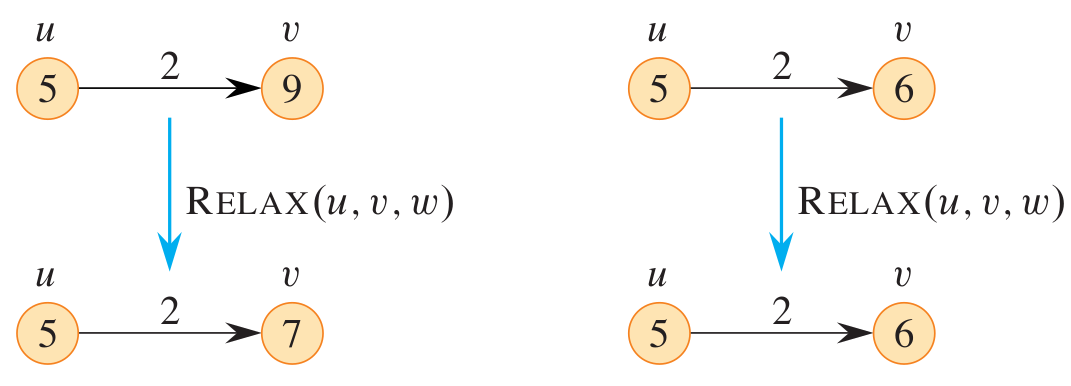
\includegraphics[width=0.7\textwidth]{figs/chap07/610-relaxation}
\end{figure}
\end{itemize}
\end{frame}


\begin{frame}{‌کوتاهترین مسیر از یک مبدأ}
\begin{itemize}\itemr
\item[-]
دو الگوریتم مهم برای محاسبه کوتاهترین مسیر عبارتند از الگوریتم بلمن فورد و الگوریتم دایکسترا.
\item[-]
در الگوریتم بلمن فورد هر یال
\m{|V| - 1}
بار آزادسازی می‌شود، اما در الگوریتم دایکسترا هر یال فقط یک بار آزادسازی می‌شود.
\item[-]
در الگوریتم بلمن‌فورد وزن یال‌ها می‌توانند منفی نیز باشد، اما الگوریتم دایکسترا تنها گراف‌هایی با وزن یال مثبت را می‌پذیرد.
وزن یال منفی می‌تواند کاربردهای متنوعی داشته باشد. برای مثال، اگر یک خودروی برقی را در نظر بگیریم که در جاده‌هایی با شیب منفی شارژ می‌شود و در جاده‌هایی با شیب مثبت انرژی مصرف می‌کند، می‌توانیم شیب جاده را به عنوان وزن یال‌های گراف در نظر بگیریم.
\end{itemize}
\end{frame}